Die Niederländische Bank hat 2018 eine Studie über die Auswirkungen des niederländischen Bargeldsystems auf die Umwelt und den Klimawandel aus 2015 veröffentlicht. In dieser Studie wird ein Life Cycle Assessment in Kombination mit der ReCiPe 2008 (H) Methode durchgeführt. Das Ziel der Studie ist es, einen quantitativen Einblick in die Auswirkungen des niederländischen Bargeldsystems auf die Umwelt zu erhalten und die Ergebnisse der Studie zu veröffentlichen. Für den Untersuchungsrahmen wurden zwei funktionale Einheiten bestimmt. Die erste Einheit ist das gesamte niederländische Bargeldsystem mit allen Transaktionen aus 2015. Die zweite funktionale Einheit ist eine durchschnittliche Bargeldzahlung in den Niederlanden in 2015, welche hinzugefügt wurde, um am Ende eine einzelne Bargeldzahlung mit einer einzelnen Debitkartenzahlung zu vergleichen\citebib{nlbank}{S.4}{vgl. }.\\
Für die Sachbilanz wurde das Bargeldsystem in fünf Subsysteme unterteilt. Die Produktion von Banknoten, die Produktion von Münzen, die operative Phase, die End-of-Life-Phase der Banknoten und die End-of-Life-Phase der Münzen. Diese Subsysteme wurden in verschiedene Prozesse unterteilt, welche dann bei der Datenerhebung betrachtet wurden, um die Umweltwirkung der Subsysteme zu berechnen. Die genaue Unterteilung ist in der nachfolgenden Grafik zu erkennen\citebib{nlbank}{S.5ff.}{vgl. }.
\FloatBarrier
\begin{figure}[ht!]
    \centering
    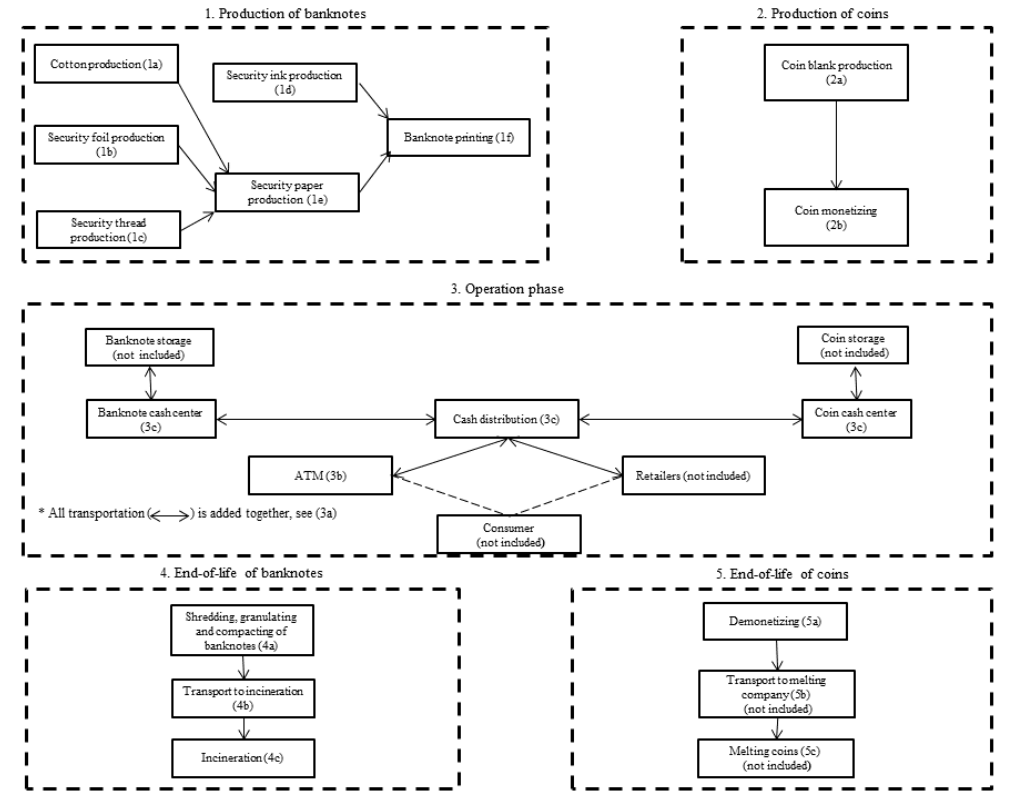
\includegraphics[width=\textwidth]{quellen/bgsys.png}
    \caption[Der Lebenszyklus des Bargeldsystems in fünf Subsystemen]{Der Lebenszyklus des Bargeldsystems in fünf Subsystemen (\textit{Hanegraaf et al.}, S.5)}
\end{figure}
\FloatBarrier
\noindent Für die Wirkungsabschätzung wurde die ReCiPe (H) Methode verwendet, um die Umweltwirkung in Ecopoints zu berechnen. Dabei kam die Studie auf ein Ergebnis von 2,35 MPt (Millionen Ecopoints) für das gesamte niederländische Bargeldsystem. Der größte Anteil der Ecopoints ergab sich aus der operativen Phase mit 1,49 MPt. Danach kam die Produktion der Münzen mit 0,75 MPt und dann die Produktion der Banknoten mit 0,12 MPt. Die beiden End-of-Life-Phasen hatten einen insignifikanten Einfluss auf die Umwelt. Eine einzelne Bargeldzahlung belief sich auf 631 \begin{math}\mu Pt\end{math}\citebib{nlbank}{S.15}{vgl. }.\\
In der Auswertung wurden unter anderem verschiedene Szenarien diskutiert, welche Maßnahmen getroffen werden könnten, um die Auswirkungen auf die Umwelt zu reduzieren und wie sich diese Maßnahmen auf die Ecopoints niederschlagen würden\citebib{nlbank}{S.19ff.}{vgl. }.